% Convert with command:
% convert -density 300 pic.pdf -quality 90 pic.png
\documentclass[crop,tikz,border=0pt]{standalone}
\usetikzlibrary{arrows.meta, fit}
% \usetikzlibrary{fit}
\begin{document}
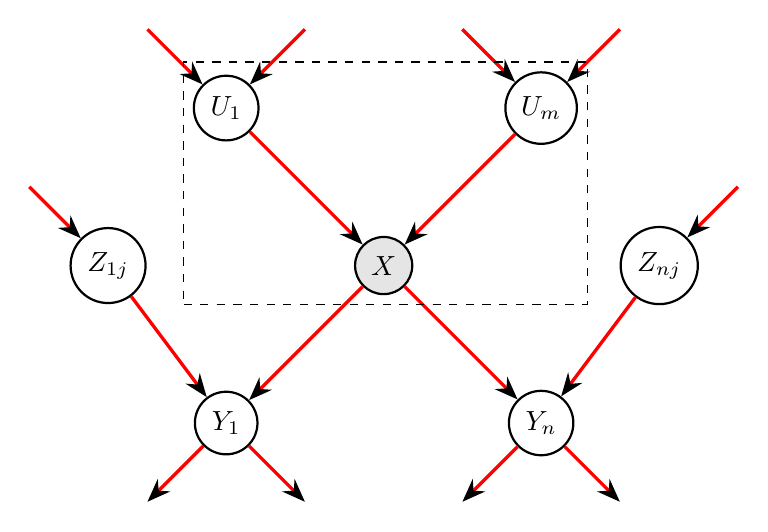
\begin{tikzpicture}

\begin{scope}[every node/.style={circle,thick,draw}]
    \node (u1) at (0, 0) [shape=circle, fill=white] {$U_1$};
    \node (um) at (4, 0) [shape=circle, fill=white] {$U_m$};

    \node (x) at (2, -2) [shape=circle, fill=gray!20] {$X$};

    \node (z1) at (-1.5, -2) [shape=circle, fill=white] {$Z_{1j}$};
    \node (zn) at (5.5, -2) [shape=circle, fill=white] {$Z_{nj}$};

    \node (y1) at (0, -4) [shape=circle, fill=white] {$Y_1$};
    \node (yn) at (4, -4) [shape=circle, fill=white] {$Y_n$};
\end{scope}

\begin{scope}[>={Stealth[black]},
            %   every node/.style={fill=white,rectangle,above},
              every edge/.style={draw=red,very thick}]
    \path [->] (-1, 1) edge node {} (u1);
    \path [->] (1, 1) edge node {} (u1);
    \path [->] (u1) edge node {} (x);

    \path [->] (3, 1) edge node {} (um);
    \path [->] (5, 1) edge node {} (um);
    \path [->] (um) edge node {} (x);

    \path [->] (x) edge node {} (y1);
    \path [->] (x) edge node {} (yn);

    \path [->] (-2.5, -1) edge node {} (z1);
    \path [->] (z1) edge node {} (y1);

    \path [->] (6.5, -1) edge node {} (zn);
    \path [->] (zn) edge node {} (yn);

    \path [->] (y1) edge node {} (-1, -5);
    \path [->] (y1) edge node {} (1, -5);

    \path [->] (yn) edge node {} (3, -5);
    \path [->] (yn) edge node {} (5, -5);
\end{scope}

\node[draw,dashed,fit=(x) (u1) (um)] {};

\end{tikzpicture}

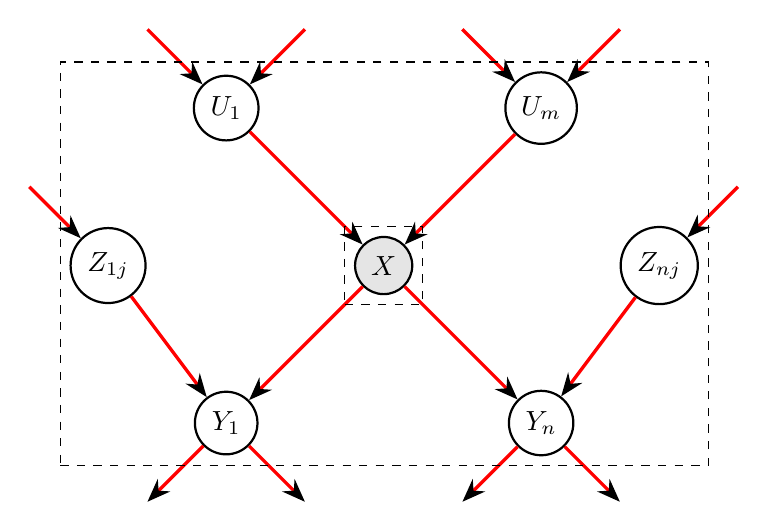
\begin{tikzpicture}

\begin{scope}[every node/.style={circle,thick,draw}]
    \node (u1) at (0, 0) [shape=circle, fill=white] {$U_1$};
    \node (um) at (4, 0) [shape=circle, fill=white] {$U_m$};

    \node (x) at (2, -2) [shape=circle, fill=gray!20] {$X$};

    \node (z1) at (-1.5, -2) [shape=circle, fill=white] {$Z_{1j}$};
    \node (zn) at (5.5, -2) [shape=circle, fill=white] {$Z_{nj}$};

    \node (y1) at (0, -4) [shape=circle, fill=white] {$Y_1$};
    \node (yn) at (4, -4) [shape=circle, fill=white] {$Y_n$};
\end{scope}

\begin{scope}[>={Stealth[black]},
            %   every node/.style={fill=white,rectangle,above},
              every edge/.style={draw=red,very thick}]
    \path [->] (-1, 1) edge node {} (u1);
    \path [->] (1, 1) edge node {} (u1);
    \path [->] (u1) edge node {} (x);

    \path [->] (3, 1) edge node {} (um);
    \path [->] (5, 1) edge node {} (um);
    \path [->] (um) edge node {} (x);

    \path [->] (x) edge node {} (y1);
    \path [->] (x) edge node {} (yn);

    \path [->] (-2.5, -1) edge node {} (z1);
    \path [->] (z1) edge node {} (y1);

    \path [->] (6.5, -1) edge node {} (zn);
    \path [->] (zn) edge node {} (yn);

    \path [->] (y1) edge node {} (-1, -5);
    \path [->] (y1) edge node {} (1, -5);

    \path [->] (yn) edge node {} (3, -5);
    \path [->] (yn) edge node {} (5, -5);
\end{scope}

\node[draw,dashed,fit=(x) (u1) (um) (y1) (yn) (z1) (zn)] {};
\node[draw,dashed,fit=(x)] {};

\end{tikzpicture}
\end{document}
